\section{Zielsetzung}
    \label{sec:Zielsetzung}

    Ziel des Versuch ist es, die temperaturabhängige dynamische Viskosität $\eta(T)$ von Wasser zu bestimmen. Dazu werden verschiedene Messungen
    mit einem Kugelfall-Viskosimeter nach Höppler durchgeführt. Zusätzlich wird die Reynoldzahl berechnet, um zu bestimmen wie turbulent die Strömung
    des Wassers verläuft.

\section{Theorie}
    \label{sec:Theorie}
    Wenn sich ein Objekt durch ein anderes Material bewegt (gasförmig oder flüssig), wirkt eine Reibungskraft $\vec{F}_{\symup{R}}$ entgegen der
    Bewegungsrichtung auf diesen Körper. Die Stärke der Kraft hängt von der Berührungsfläche der Flüssigkeit/Gas mit dem Körper und der
    Geschwindigkeit $\vec{v}$ des Objekts ab. \\
    Bei zähen Flüssigkeiten wirkt neben der Reibungskraft $\vec{F}_{\symup{R}}$ beim Fall auch die Schwerkraft $\vec{F}_g$ und die Auftriebskraft $\vec{F}_{\symup{A}}$. Dies 
    muss bei Rechnungen berücksichtigt werden.\\
    Bei sphärischen Objekten in Fluiden lässt sich das Gesetz von Stokes anwenden, welches die Reibungskraft von Kugeln in Abhängigkeit von dem Objektradius,
    der dynamischen Viskosität der Flüssigkeit und der Geschwindigkeit der Kugel beschreibt. Die Formel der Stokesschen Reibungskraft ist gegeben durch
    \begin{equation}
        \label{eqn:Stokes}
        \vec{F}_{\symup{R}} = 6 \, \pi \, \eta \, \vec{v} \, r \, .
    \end{equation}
    Das $\eta$ steht in der Formel für die dynamische Viskosität des Fluids, eine temperaturabhängige Materialeigenschaft. Sie lässt sich einmal durch die Formel
    \begin{equation}
        \label{eqn:etaK}
        \eta = K \, (\rho_{\symup{K}} - \rho_{\symup{Fl}}) \cdot t
    \end{equation}
    und durch die Andradsche Gleichung
    \begin{equation}
        \label{eqn:Andrad}
        \eta(T) = A \, \exp{\left(\frac{B}{T}\right)}
    \end{equation}
    beschreiben.\\
    Bei \autoref{eqn:etaK} handelt es sich um eine Formel, die es ermöglicht die Viskosität beim Versuch mit dem Kugelfall-Viskosimeter nach Höppler zu errechnen.
    Das $K$ ist eine Apparaturkonstante, die sich aus der Kugelgeometrie und der Fallhöhe zusammensetzt. $\rho_{\symup{Fl}}$ ist die Dichte der Flüssigkeit und $\rho_{\symup{K}}$ die Dichte
    des Kugel. $t$ beschreibt die Fallzeit der Kugel in dem Viskosimeter.\\
    Die Andradsche Gleichung (\ref{eqn:Andrad}) beschreibt die Viskosität in Abhängigkeit der Temperatur. Die Konstanten $A$ und $B$ lassen sich durch \autoref{eqn:etaK}
    herleiten.\\
    Da die Formel zur Stokesschen Reibungskraft nur bei möglichst laminaren (und somit nicht turbulenten) Strömungen anwendbar ist, wird während des Versuchsdurchführung die
    Reynoldzahl der Strömung untersucht. Die Reynoldzahl gibt Aussage darüber, wie laminar eine Strömung ist. Sie berechnet sich zu
    \begin{equation}
        \label{eqn:Reynoldzahl}
        Re := \frac{\rho_{\symup{Fl}}\,\bar{v}\,d}{\eta}.
    \end{equation}
    Das $\eta$ ist hier wie zuvor die Viskosität der Flüssigkeit, $d$ der Durchmesser des Rohres des Fall-Viskosimeters, $\bar{v}$ die mittlere Geschwindigkeit der Kugel und
    $\rho_{\symup{Fl}}$ die Dichte der Flüssigkeit.\\
    Um später die Dichte $\rho_{\symup{K}}$ der Kugel zu berechnen benötigen wir die Formel
    \begin{equation}
        \label{eqn:KugelDichte}
        \rho_{\symup{K}} = \frac{M}{V} = \frac{4}{3 \,\pi \, r^3} \cdot M.
    \end{equation}

\subsection{Kugelfall-Viskosimeter nach Höppler}

\begin{wrapfigure}{r}{5.5cm}
    \centering
    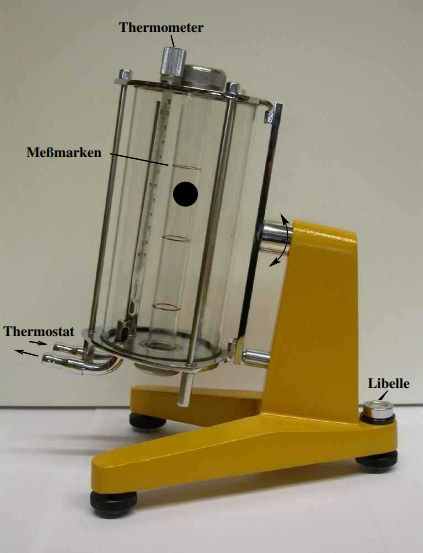
\includegraphics[width=5.5cm]{Kugelfall.png}
    \caption{Kugelfall-Viskosimeter nach Höppler \cite{anleitung107}}
    \label{Abb:Kugelfall}
\end{wrapfigure}

Zur Versuchsdurchführung wird ein Kugelfall-Viskosimeter nach Höppler verwendet. Das Viskosimeter besteht aus einem Fallrohr, welches von
einem breiteren Glasrohr umgeben ist. Das breitere Rohr ist mit Wasser gefüllt und an ein Thermostat angeschlossen, wodurch sich die Temperatur regeln
lässt. Das Fallrohr wird nur indirekt durch das äußere Rohr erhitzt um zusätzliche Turbulenzen zu vermeiden.\\
Das Fallrohr hat zwei verschließbare Öffnungen und drei Markierungen auf der Glaswand, welche jeweils 5\,$\unit{cm}$ auseinander liegen. Das Rohr wird
leicht geneigt, um die Strömung des Wassers möglichst laminar zu halten und Wirbel zu vermeiden.\\
Für die Messungen wird das Rohr mit Wasser gefüllt und eine geringfügig kleinere Kugel in das Rohr gegeben. Hierbei muss darauf geachtet werden, dass sich keine 
Blasen bilden, da dies zu zusätzlicher Reibung führt. Damit die Kugel nicht nach jedem Fall wieder rausgenommen werden muss, lässt sich das Fallrohr seitlich um 
$\mathrm{180^{\circ}}$ drehen.\\

\subsection{Vorbereitungsaufgaben}

\textbf{Wann wird eine Strömung als laminar bezeichnet?} \\
Eine Strömung ist laminar, wenn keine sichbaren Turbulenzen bzw. Wirbel auftreten und die Flüssigkeit somit in Schichten strömt, die sich nicht durch die Wirbel
miteinander vermischen.\\ \\
\textbf{Wie lautet die dynamische Viskosität von destillierten Wasser als Funktion der Temperatur?}\\
Nach intensiver Recherche lässt sich selbst in den Büchern des Literaturverzeichnis' keine temperaturabhängige Funktion der dynamischen Viskosität von destillierten Wasser 
finden. Die allgemeine Funktion lässt sich in \autoref{eqn:Andrad} wiederfinden. In den vorgeschlagenen Büchern ist ein Wert für die dynamische Viskosität gegeben
durch $\eta(20 \, ^{\circ}\unit{C}) = 1,005 \cdot \mathrm{10^{-3} \, Pa \, \, s}$.\\ \\
\textbf{Wie lautet die temperaturabhängige Dichte von destillierten Wasser?}\\
Die temperaturabhängige Dichte von Wasser lässt sich durch die ideale Gasgleichung herleiten und ist abhängig vom Umgebungsdruck $p$, der Gesamtmasse $M$, der Gaskonstante
$R$ und der Temperatur $T$ in Kelvin. Sie ist gegeben durch
\begin{equation}
    \label{eqn:tempDichte}
    \rho(T) = \frac{M}{V} = \frac{p \cdot M}{R \cdot T}.
\end{equation}